\documentclass[a4paper,11pt,fleqn,twoside,notitlepage]{report}
\usepackage[]{graphicx}\usepackage[]{color}
%% maxwidth is the original width if it is less than linewidth
%% otherwise use linewidth (to make sure the graphics do not exceed the margin)
\makeatletter
\def\maxwidth{ %
  \ifdim\Gin@nat@width>\linewidth
    \linewidth
  \else
    \Gin@nat@width
  \fi
}
\makeatother

\definecolor{fgcolor}{rgb}{0.345, 0.345, 0.345}
\newcommand{\hlnum}[1]{\textcolor[rgb]{0.686,0.059,0.569}{#1}}%
\newcommand{\hlstr}[1]{\textcolor[rgb]{0.192,0.494,0.8}{#1}}%
\newcommand{\hlcom}[1]{\textcolor[rgb]{0.678,0.584,0.686}{\textit{#1}}}%
\newcommand{\hlopt}[1]{\textcolor[rgb]{0,0,0}{#1}}%
\newcommand{\hlstd}[1]{\textcolor[rgb]{0.345,0.345,0.345}{#1}}%
\newcommand{\hlkwa}[1]{\textcolor[rgb]{0.161,0.373,0.58}{\textbf{#1}}}%
\newcommand{\hlkwb}[1]{\textcolor[rgb]{0.69,0.353,0.396}{#1}}%
\newcommand{\hlkwc}[1]{\textcolor[rgb]{0.333,0.667,0.333}{#1}}%
\newcommand{\hlkwd}[1]{\textcolor[rgb]{0.737,0.353,0.396}{\textbf{#1}}}%

\usepackage{framed}
\makeatletter
\newenvironment{kframe}{%
 \def\at@end@of@kframe{}%
 \ifinner\ifhmode%
  \def\at@end@of@kframe{\end{minipage}}%
  \begin{minipage}{\columnwidth}%
 \fi\fi%
 \def\FrameCommand##1{\hskip\@totalleftmargin \hskip-\fboxsep
 \colorbox{shadecolor}{##1}\hskip-\fboxsep
     % There is no \\@totalrightmargin, so:
     \hskip-\linewidth \hskip-\@totalleftmargin \hskip\columnwidth}%
 \MakeFramed {\advance\hsize-\width
   \@totalleftmargin\z@ \linewidth\hsize
   \@setminipage}}%
 {\par\unskip\endMakeFramed%
 \at@end@of@kframe}
\makeatother

\definecolor{shadecolor}{rgb}{.97, .97, .97}
\definecolor{messagecolor}{rgb}{0, 0, 0}
\definecolor{warningcolor}{rgb}{1, 0, 1}
\definecolor{errorcolor}{rgb}{1, 0, 0}
\newenvironment{knitrout}{}{} % an empty environment to be redefined in TeX

\usepackage{alltt}
\newcommand{\SweaveOpts}[1]{}  % do not interfere with LaTeX
\newcommand{\SweaveInput}[1]{} % because they are not real TeX commands
\newcommand{\Sexpr}[1]{}       % will only be parsed by R


\usepackage[utf8]{inputenc}
\usepackage[margin=2.5cm]{geometry}
\usepackage{graphicx}
\usepackage[T1]{fontenc}
\usepackage{amsmath}

\usepackage{csquotes}
\usepackage[english]{babel}
\usepackage{float}
\usepackage{caption}
\usepackage{makecell}
\usepackage{hyperref}
\usepackage{bm}
\usepackage{newfloat}
\usepackage{amsfonts}

\usepackage[linesnumbered,lined,boxed,commentsnumbered]{algorithm2e}

\usepackage{tikz}
%\usetikzlibrary{calc,trees,positioning,arrows,chains,shapes.geometric,%
%    decorations.pathreplacing,decorations.pathmorphing,shapes,%
%    matrix,shapes.symbols}

% \tikzstyle{punktchain} = [rectangle,
%     rounded corners,
%     draw=black, very thick,
%     text width=10em,
%     minimum height=3em,
%     text centered,
%     on chain,
%     top color=white,
%     bottom color=blue!20]
    
%\tikzset{arrow} = [thick,->,>=stealth]
\usepackage{fancyhdr}
\setlength{\headheight}{15pt}

\pagestyle{fancy}
\renewcommand{\chaptermark}[1]{ \markboth{#1}{} }
\renewcommand{\sectionmark}[1]{ \markright{#1}{} }

\fancyhf{}
\fancyfoot[CE,CO]{\thepage}
\fancyhead[LE]{\textit{ \nouppercase{\leftmark}} }
\fancyhead[LO]{\textit{ \nouppercase{\rightmark}} }
%\fancyhead[RE,RO]{Erik Thors\'{e}n, \href{mailto:Ethorsn@gmail.com}{Ethorsn@gmail.com} }
\fancypagestyle{plain}{ %
\fancyhf{} % remove everything
  \renewcommand{\headrulewidth}{0pt} % remove lines as well
  \renewcommand{\footrulewidth}{0pt}
}

\DeclareFloatingEnvironment[placement={!ht},name=List]{mylist}

\usepackage[
citestyle=authoryear,
bibstyle=authoryear,
backend=bibtex
]{biblatex}

\addbibresource{REFERENCES.bib}
\title{Quality control in next-generation sequencing quality control data?}
\author{Erik Thors\'{e}n \thanks{Postal adress: Mathematical Statistics, Stockholm University, SE-106 91, Sweden. E-mail: Ethorsn@gmail.com. Supervisor: Taras Bodnar and Johan Dahlberg}}
\date{\today}
%\newcommand{\opn}[1]{\operatorname{#1}}
\raggedbottom


\begin{document}

\begin{knitrout}
\definecolor{shadecolor}{rgb}{0.969, 0.969, 0.969}\color{fgcolor}\begin{kframe}
\begin{alltt}
\hlkwd{library}\hlstd{(Rcpp)}
\hlkwd{library}\hlstd{(RcppArmadillo)}
\hlkwd{library}\hlstd{(dplyr)}
\end{alltt}


{\ttfamily\noindent\itshape\color{messagecolor}{\#\# \\\#\# Attaching package: 'dplyr'}}

{\ttfamily\noindent\itshape\color{messagecolor}{\#\# The following objects are masked from 'package:stats':\\\#\# \\\#\#\ \ \ \  filter, lag}}

{\ttfamily\noindent\itshape\color{messagecolor}{\#\# The following objects are masked from 'package:base':\\\#\# \\\#\#\ \ \ \  intersect, setdiff, setequal, union}}\begin{alltt}
\hlkwd{library}\hlstd{(ggplot2)}
\hlkwd{sourceCpp}\hlstd{(}\hlstr{"../FunctionsAndRcpp/RcppSimulateARL0.cpp"}\hlstd{)}
\hlkwd{load}\hlstd{(}\hlstr{"../Data/ICdata.Rdata"}\hlstd{)}
\hlkwd{load}\hlstd{(}\hlstr{"../Data/meanH.Rdata"}\hlstd{)}

\hlstd{K} \hlkwb{<-} \hlnum{100}
\hlstd{OrgOrder} \hlkwb{<-} \hlkwd{colnames}\hlstd{(TransformedData)}
\hlcom{# divide by a constant!}
\hlstd{TransformedData[,}\hlnum{1}\hlopt{:}\hlkwd{ncol}\hlstd{(TransformedData)} \hlopt \hlkwd{grep}\hlstd{(}\hlstr{"mean"}\hlstd{,OrgOrder)]} \hlkwb{<-} \hlstd{TransformedData[,}\hlnum{1}\hlopt{:}\hlkwd{ncol}\hlstd{(TransformedData)} \hlopt \hlkwd{grep}\hlstd{(}\hlstr{"mean"}\hlstd{,OrgOrder)]}\hlopt{/}\hlstd{K}

\hlstd{mu0} \hlkwb{<-} \hlkwd{colMeans}\hlstd{(TransformedData)}
\hlstd{Sigma0} \hlkwb{<-} \hlkwd{var}\hlstd{(TransformedData)}

\hlstd{h} \hlkwb{<-} \hlstd{H_Listmean[[}\hlnum{1}\hlstd{]]}\hlopt{$}\hlstd{Intervals} \hlopt \hlkwd{na.omit}\hlstd{()} \hlopt \hlkwd{tail}\hlstd{(}\hlnum{1}\hlstd{)} \hlopt \hlkwd{mean}\hlstd{()}
\hlstd{k} \hlkwb{<-} \hlnum{0.3}
\end{alltt}
\end{kframe}
\end{knitrout}
In this section we will shortly show some benchmarks of the \textt{SimulateARL0} function implemented in Rcpp used in this thesis. Almost every other function used for the calculations in this thesis are implemented in Rcpp. We will use the following settings for our simulations 
\begin{itemize}
\item The in control mean and covariance matrix previously estimated from data
\item A allowance constant equal to $0.3$
\item The control limit $2580.242$
\item The number of threads was held constant, equal to 7. 
\end{itemize}
The number of simulations N=$\{10^2,10^3,10^4,10^5\}$. Each simulation is performed 10 times and the average time is taken as the benchmark for this specific setting. 
The test system was a Intel\textregistered Core i7-4770S@3.1Ghz with 16Gb system RAM running Ubuntu 14.04.4.
\begin{knitrout}
\definecolor{shadecolor}{rgb}{0.969, 0.969, 0.969}\color{fgcolor}\begin{kframe}
\begin{alltt}
\hlkwd{library}\hlstd{(microbenchmark)}
\hlstd{benchman} \hlkwb{<-} \hlkwd{microbenchmark}\hlstd{(}\hlstr{"1e1"}\hlstd{=}\hlkwd{SimulateARL0}\hlstd{(}\hlnum{1e1}\hlstd{, h,k,mu0,Sigma0,}\hlnum{7}\hlstd{),}
                           \hlstr{"1e2"}\hlstd{=}\hlkwd{SimulateARL0}\hlstd{(}\hlnum{1e2}\hlstd{, h,k,mu0,Sigma0,}\hlnum{7}\hlstd{),}
                           \hlstr{"1e3"}\hlstd{=}\hlkwd{SimulateARL0}\hlstd{(}\hlnum{1e3}\hlstd{, h,k,mu0,Sigma0,}\hlnum{7}\hlstd{),}
                           \hlstr{"1e4"}\hlstd{=}\hlkwd{SimulateARL0}\hlstd{(}\hlnum{1e4}\hlstd{, h,k,mu0,Sigma0,}\hlnum{7}\hlstd{),}
                           \hlstr{"1e5"}\hlstd{=}\hlkwd{SimulateARL0}\hlstd{(}\hlnum{1e5}\hlstd{, h,k,mu0,Sigma0,}\hlnum{7}\hlstd{),}
                           \hlkwc{times}\hlstd{=}\hlnum{10}\hlstd{)}
\end{alltt}
\end{kframe}
\end{knitrout}

\begin{knitrout}
\definecolor{shadecolor}{rgb}{0.969, 0.969, 0.969}\color{fgcolor}\begin{kframe}
\begin{alltt}
\hlkwd{library}\hlstd{(ggplot2)}
\hlkwd{autoplot}\hlstd{(benchman)} \hlopt{+}
  \hlkwd{theme_bw}\hlstd{()}
\end{alltt}
\end{kframe}\begin{figure}
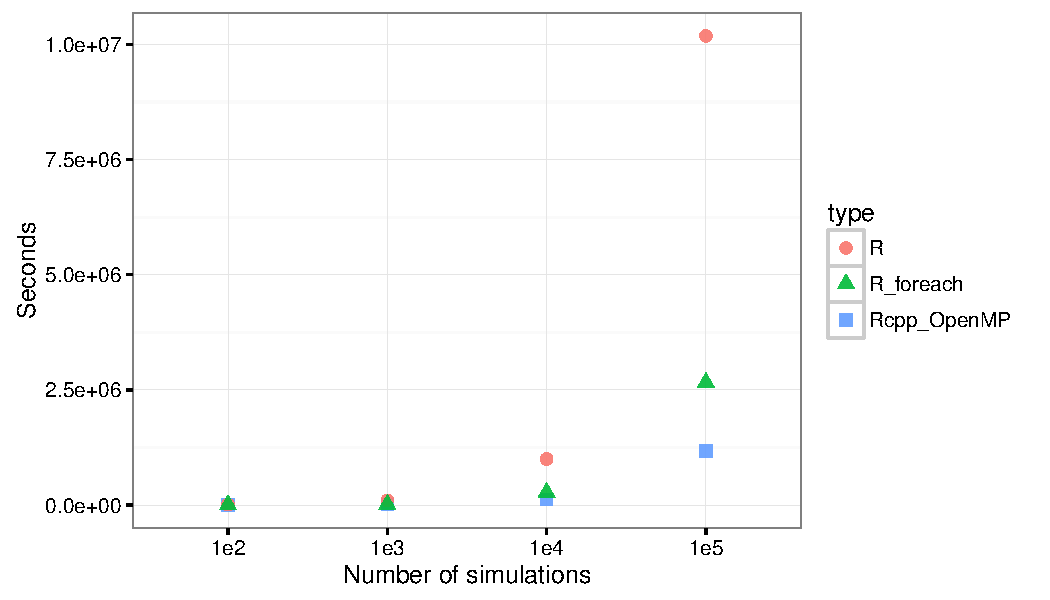
\includegraphics[width=\maxwidth]{figure/BenchmarkFigure-1} \caption[Benchmark of the SimulateARL0 function, implemented in Rcpp together with OpenMP]{Benchmark of the SimulateARL0 function, implemented in Rcpp together with OpenMP. }\label{fig:BenchmarkFigure}
\end{figure}


\end{knitrout}
The C++ (Rcpp) code for the \texttt{SimulateARL0} function is presented below.
\begin{knitrout}
\definecolor{shadecolor}{rgb}{0.969, 0.969, 0.969}\color{fgcolor}\begin{kframe}
\begin{alltt}
#include <RcppArmadillo.h>
#include <math.h>

#ifdef _OPENMP
#include <omp.h>
#endif

using namespace std;
using namespace Rcpp;
using namespace arma;


// [[Rcpp::plugins(openmp)]]
// [[Rcpp::depends(RcppArmadillo)]]

rowvec SnewFun(rowvec Snew, rowvec Sold, rowvec mu0, mat Sigma0, double k) \{
  //inits
  rowvec SNEW;
  mat SigmaInv = Sigma0.i();
  
  colvec Y = solve(Sigma0, trans(Snew+Sold-mu0));
  // statistical distance, Mahalanobis distance.
  double D = pow(as_scalar((Snew+Sold-mu0)*Y),0.5);
  if (D>k)\{
    double Dinv = as_scalar(pow(D,-1));
    SNEW = (Snew+Sold-mu0)*(1-k*Dinv);
  \}else\{
    int length = Sigma0.n_rows;
    SNEW = zeros<rowvec>(length);
  \};
  return SNEW;
\}

double CFun(rowvec Snew, rowvec Sold, rowvec mu0, mat Sigma0, double k)\{
  //inits
  double C;
  rowvec SNEW;
  mat SigmaInv = Sigma0.i();
  
  colvec Y = solve(Sigma0, trans(Snew+Sold-mu0));
  // statistical distance, Mahalanobis distance.
  double D = pow(as_scalar((Snew+Sold-mu0)*Y),0.5);
  if (D>k)\{
    double Dinv = as_scalar(pow(D,-1));
    SNEW = (Snew+Sold-mu0)*(1-k*Dinv);
    C = as_scalar(SNEW * SigmaInv * SNEW.t());
  \}else\{
    C = 0;
  \};
  return C;
\}

// For simulating ONE multivariate normal obs.
rowvec mvrnormArma(rowvec mu, mat sigma) \{
  int ncols = sigma.n_cols;
  rowvec Y = randn<rowvec>(ncols);
  rowvec ret = mu + Y * chol(sigma);
  return ret;
\}

// function for taking the midpoint
inline double midpoint(double val1, double val2) \{
  return (val1 + val2) / 2;
\}

// Simulate ARL0 based on k and h in parallel using open MP. 
// [[Rcpp::export]]
rowvec SimulateARL0(SEXP n, SEXP h, SEXP k, SEXP mu0, SEXP Sigma0, SEXP No_threads) \{
  // inits
  int N = as<int>(n);
  double H = as<double>(h);
  double K = as<double>(k);
  int Nthread = as<int>(No_threads);
  
  rowvec Mu = as<rowvec>(mu0);
  
  mat Sigma = as<mat>(Sigma0);
  rowvec VecReturn = zeros<rowvec>(N);
  
  size_t l; 
  int counter;
  double Cstat;
  rowvec S_old(Sigma.n_cols), Sims(Sigma.n_cols);
  
  class InvalidDim_exception: public std::exception \{\};
  class NegParams_exception: public std::exception \{\};
                                                     
  try\{
    if (Sigma.n_cols != Mu.size() || Sigma.n_rows != Mu.size())
    \{
      // Sigma, Mu and Mu1 does not have the same dimensions.
      throw InvalidDim_exception();
    \}
    else if (K < 0 || H < 0)
    \{
      // k or h is negative
      throw NegParams_exception();
    \}
    else
    \{
      printf("Inits done! Starting simulations. \textbackslash{}n");
    \}
    
    /*
     * The addition of #pragma from OpenMP does everything in the background.
     * So the following code is in parallel, using Nthread (num_threads(Nthread)) threads.
     */
#pragma omp parallel for num_threads(Nthread) shared(VecReturn) private(l, counter, Cstat, S_old, Sims) firstprivate(H, K, Mu, Sigma)
      for (l = 0; l < N;++l)\{
        // Inits for a run
        counter = 1;
        Cstat = 0;
        S_old = zeros<rowvec>(Sigma.n_cols);
        // simulating the expectation.
        for (int k=0; k<10000; ++k)\{
          Sims = mvrnormArma(Mu, Sigma);
          // Use MCUSUM scheme, first update Cstat then S_old.
          Cstat = CFun(Sims, S_old, Mu, Sigma, K);
          S_old = SnewFun(Sims, S_old, Mu, Sigma, K);
          if (Cstat > H)\{break;\};
          counter += 1;
        \};
        VecReturn(l) = counter;  
      \};
  \}
  catch(NegParams_exception e)\{
    // add dimensions or print values of parameters
    cerr << "Negative values of the control limit (h) or allowance constant (k) are not allowed." << endl;
    throw e;
    rowvec ret;
    return ret;
  \}
  catch(InvalidDim_exception e)\{
    // add dimensions or print values of parameters
    cerr << "The dimensions of the mean vector (mu0 or mu1) and Covariance matrix are not the same." << endl;
    rowvec ret;
    return ret;
  \}
  return VecReturn;
\}

\end{alltt}
\end{kframe}
\end{knitrout}
\end{document}
